\partimage[width=0.8\columnwidth]{Figures/PartImages/FigCh1.png}
\part{La génération d'harmoniques d'ordre élevé : bases théoriques et expérimentales}
\label{PA:GHOE}
\chapter{Théorie de la génération d'harmoniques d'ordre élevé}
La génération d'harmoniques d'ordre élevé (GHOE) est un phénomène de champ fort observé pour la première fois en 1987 par \mycite{mcphersonJOSAB1987} et \mycite{FerrayJPB1988}. En soumettant un gaz d'atomes ou de molécules à un champ laser dans le bon régime d'intensité et d'accord de phase, on assiste à la génération des harmoniques de la fréquence optique du laser de génération. De manière remarquable, ce processus est non-perturbatif : l'intensité de la $q$-ième harmonique n'évolue pas en $I_0^q$, où $I_0$ est l'intensité du laser incident. C'est ce phénomène de GHOE qui nous a servi de base à l'étude des transferts de moments angulaires du visible vers l'XUV dans l'intégralité de cette thèse. Dans cette partie, nous présentons d'abord la théorie le décrivant, avant d'expliquer comment il est mis en œuvre expérimentalement dans le cas le plus simple.

En 1993, \mycite{SchaferPRL1993} et \mycite{CorkumPRL1993}\footnote{Ces travaux ont eu un précurseur significatif : le modèle de "l'antenne atomique" \mycite{kuchiev1987}.} proposent un modèle semi-classique simple expliquant le processus de génération d'harmoniques d'ordre élevé. Il permet une compréhension qualitative du phénomène.

\section{Modèle à 3 étapes}
\label{sec:threestep}
Le modèle proposé se décompose en trois étapes. On commence par soumettre le gaz cible au champ électrique d'un faisceau laser intense, ce qui abaisse la barrière de potentiel des atomes\footnote{Par commodité on parlera d'atomes, en gardant à l'esprit qu'il est aussi possible d'utiliser des molécules.} du gaz. Le champ laser est choisi pour abaisser largement cette barrière quand il est maximal, sans toutefois la supprimer. Un paquet d'onde électronique (POE) peut alors être émis par \textit{ionisation tunnel}. Ensuite, ce POE est accéléré par le champ laser dans le continuum. Quand le champ laser change de signe, il est freiné puis réaccéléré vers son atome parent. Enfin, lorsque le POE passe à proximité de l'atome, il a une certaine probabilité de recombiner sur l'état fondamental. L'énergie acquise lors de la propagation dans le continuum est alors restituée sous forme de photons qui, comme on le verra, ont une énergie dans l'extrême ultraviolet (XUV). Dans les paragraphes suivants nous décrivons successivement ces trois étapes.

\subsection{Première étape : ionisation tunnel}
Considérons un atome isolé dans son état fondamental. Un électron dans cet état est soumis au potentiel coulombien du noyau, de la forme\footnote{On utilise les unités atomiques.} $V_0 = -1/r$ (figure \ref{fig:ionization}.a). L'énergie du niveau fondamental est égale à l'opposée du potentiel d'ionisation de l'atome considéré, par exemple $-I_p=-15.8$ eV pour l'argon, gaz communément utilisé en GHOE. On ajoute un champ électrique polarisé linéairement, que l'on note $\bm{E(t)} = E_x \cos(\omega_0 t)\bm{e}_x$, où $\bm{e}_x$ et $\omega_0$ sont respectivement l'axe de polarisation et la fréquence angulaire du champ. Le potentiel ressenti par l'électron devient :
\begin{equation}
V(x,t) = V_0(x) + E(t)x.
\end{equation} 

\begin{figure}[!ht]
\centering
\def\svgwidth{\columnwidth}
\import{Figures/ThreeStep/}{potentials.pdf_tex}
\caption{Potentiels ressentis par l'électron dans le cas de l'argon ($I_p = 15.8\; \text{eV} = 0.58\; \text{u.a.}$, représenté par la ligne pointillée). (a) En l'absence de champ électrique, (b) En présence d'un champ $E=0.04$ u.a., (c) En présence d'un champ $E=E_{\text{sat}}=0.084$ u.a.}
\label{fig:ionization}
\end{figure}

Comme illustré sur la figure \ref{fig:ionization}.b, la barrière de potentiel est abaissée d'un côté. Si le champ est assez fort, une partie du POE peut la traverser par effet tunnel, selon une probabilité qui dépend de la hauteur et de l'épaisseur de la barrière. Dans le cas extrême, la barrière peut être totalement supprimée (figure \ref{fig:ionization}c) et la probabilité d'ionisation est égale à 1. Ce cas est réalisé pour une intensité que l'on note $I_\text{sat}$. Considérons que le champ soit maximum à l'instant considéré : $E=E_0>0$. La barrière est donc abaissée pour $x<0$. \`A l'intensité de saturation, le maximum de la barrière de potentiel est égal à $-I_p$, obtenu en $x_0$ tel que $V'(x_0) = 0$, c'est-à-dire $x_0 = -1/\sqrt{E_0}$. On a alors $-I_p = -2\sqrt{E_0}$, soit $I_\text{sat} = I_p^4/16$. Dans des unités plus habituelles, on a $I_\text{sat}(\si{W/cm^2}) = 4\times10^9I_p(\si{eV})^4$. Le tableau \ref{tab:Isat}, tiré de \mycite{gruson}, donne les valeurs obtenues pour les gaz rares, couramment utilisés en GHOE.

\begin{table}[h!]
\begin{tabular}{|c|c|c|}
  \hline
  Gaz & $I_p (\si{eV})$ & $I_{\text{sat}}\;(10^{14}\;\si{W/cm^2})$\\
  \hline
  He & 24.58 & 14.62 \\
  Ne & 21.56 & 8.65 \\
	Ar & 15.76 & 2.47 \\
	Kr & 14.00 & 1.54\\
	Xe & 12.13 & 0.87 \\
  \hline	
\end{tabular}
\centering
\caption{Potentiel d'ionisation et éclairement de saturation de différents gaz rares. Tiré de \mycite{gruson}.}
\label{tab:Isat}
\end{table}
Pour que l'ionisation tunnel ait lieu, il faut que l'intensité utilisée soit plus faible que l'intensité de saturation, de l'ordre de $10^{14}\si{W/cm^2}$. De plus, la barrière tunnel doit être abaissée pendant une durée suffisante. Cette durée est caractérisée par le paramètre de Keldysh \mycite{keldysh}, défini par $\gamma = \sqrt{I_p/U_p}$, où $U_p = I_0 \rme^2/2\omega_0^2\epsilon_0 m \rmc$ est l'énergie pondéromotrice du champ. Pour que l'ionisation tunnel domine, $\gamma$ doit être très petit devant $1$. L'application numérique pour un laser ayant une longueur d'onde de 800 nm montre que l'intensité nécessaire est de l'ordre de ${10^{13}}\si{W/cm^2}$. La gamme d'intensité où la GHOE est possible est donc assez réduite. Pour atteindre ce régime d'intensité, on utilisera des lasers de haute énergie délivrant des impulsions courtes temporellement, de l'ordre de 10-100 fs (1 fs = $10^{-15}\;s$).

\subsection{Deuxième étape : Propagation dans le continuum et recombinaison radiative}
On considère ensuite le paquet d'onde électronique sorti du puits de potentiel coulombien. On suppose alors que sa dynamique n'est gouvernée que par le champ laser, suffisamment fort pour négliger les effets à longue portée du potentiel atomique. Le champ étant assez fort, on peut utiliser une description classique de la dynamique du POE. La seule force agissant sur l'électron est la force de Lorentz, on a donc :
\begin{equation}
m\ddot{x} = -eE_0 \cos(\omega_0 t).
\label{eq:accel_3step}
\end{equation}
Pour les conditions initiales, on note $t_i$ l'instant où le POE est ionisé, et on suppose $x(t_i) = 0$ et $\dot{x}(t_i) = 0$, c'est-à-dire que l'on néglige le mouvement à travers la barrière tunnel et que l'on suppose qu'il perd toute son énergie cinétique en la traversant. On intègre \ref{eq:accel_3step} pour obtenir :
\begin{align}
\dot{x}&=-\frac{eE_0}{m\omega_0} [\sin{(w_0t)}-\sin{(w_0t_i)}]\\
x&=\frac{eE_0}{m\omega_0^2} [\cos{(w_0t)}-\cos{(w_0t_i)}]+\frac{eE_0}{m\omega_0}\sin{(w_0t_i)}(t-t_i)
\label{eq:pos_3step}
\end{align}

L'électron oscille donc dans le champ selon la direction $\bm{e}_x$ et retourne périodiquement en $x=0$, c'est-à-dire sur son atome parent. Au voisinnage de l'atome, l'électron peut recombiner et émettre un photon. En notant $E_c$ l'énergie acquise par l'électron dans le continuum, la conservation de l'énergie à l'instant de recombinaison s'écrit :
\begin{equation}
\hbar\omega = I_p+E_c
\end{equation}
où $\omega$ est la pulsation du photon émis. L'équation \ref{eq:pos_3step} suggère que des photons peuvent être émis à chaque oscillation de l'électron autour de son atome. Toutefois, si la dynamique du POE dans la direction $x$ est bien décrite classiquement, elle l'est beaucoup moins dans la direction transverse à sa trajectoire. En pratique, le POE s'étale dans la dimension transverse au cours de sa propagation. La probabilité de recombinaison en $x=0$ diminue donc à chaque période, à tel point que seul le premier retour en $x=0$ est significatif. Ainsi, pour une intensité laser et un instant d'ionisation donnés, on a un unique instant de recombinaison $t_r$ obtenu en résolvant \ref{eq:pos_3step} pour $x=0$. On calcule alors l'énergie $E(t_r) = E_c$. Sur la figure \ref{fig:recombinaison} est tracée $E_c$ en fonction du temps pour une intensité laser de $\SI{2.5e14}{W/cm^2}$.

\begin{figure}[!ht]
\centering
\def\svgwidth{\columnwidth}
\import{Figures/ThreeStep/}{recombinaison.pdf_tex}
\caption{\'Energie à la recombinaison et instants d'ionisation et de recombinaison dans l'argon pour une intensité de $\SI{2.5e14}{W/cm^2}$. Les instants d'ionisations sont en pointillés et les instants de recombinaison sont en traits pleins. La ligne pointillée horizontale indique l'énergie maximale, appelée énergie de coupure.}
\label{fig:recombinaison}
\end{figure}

On observe que l'énergie acquise par l'électron dans le continuum présente un maximum qui vaut $E_c^{\text{max}} = 3.17 U_p$. C'est l'énergie maximale qui pourra être convertie en énergie de photon, appelée \textit{énergie de coupure}. Classiquement, on voit qu'elle correspond à la dynamique de l'électron dans le continuum. L'énergie de photon maximale sera donc $\hbar\omega = I_p+3.17 U_p$. De plus, on voit que pour chaque valeur d'énergie on a deux solutions possibles. L'électron peut donc avoir deux trajectoires différentes amenant à la même énergie à la recombinaison. On les appelle trajectoires courtes et longues, de part la longueur d'excursion de l'électron dans le continuum. Pour la trajectoire courte (resp. longue), l'énergie diminue (resp. augmente) avec l'instant d'ionisation. Les deux trajectoires convergent pour devenir indiscernables à l'énergie de coupure.

Le processus décrit ici se produit à chaque fois que le champ électrique est assez fort pour abaisser le potentiel d'un côté ou de l'autre de l'atome, c'est-à-dire à chaque maximum et minimum du champ. Il a donc une périodicité de $T/2$, où $T = 2\pi/\omega_0$ est la période du laser de génération. Cette périodicité temporelle se traduit par une périodicité de $2\omega_0$ dans le domaine fréquentiel. Pour une impulsion de génération assez longue, le spectre du rayonnement émis est donc un peigne d'harmoniques séparées de $2\omega_0$. De plus, le milieu de génération étant centro-symétrique, seules les harmoniques impaires sont émises.

Le modèle présenté ici est semi-classique : l'étape d'ionisation tunnel est décrite quantiquement, tandis que la propagation de l'électron est considérée classiquement. Il donne une image simple du processus et donne accès à des valeurs importantes telles que l'énergie de coupure et les instants d'ionisation et de recombinaison. Pour en étudier la validité, il est nécessaire de la comparer à une approche plus rigoureuse en effectuant un traitement quantique.

\section{Description quantique de la GHOE : le modèle de Lewenstein}
\label{sec:thSfa}
En 1994, Maciej Lewenstein a développé un traitement complètement quantique de la GHOE \mycite{LewensteinPRA1994}. Nous décrivons ici succinctement les bases de ce modèle. On considère un seul électron actif soumis au champ électrique $\bm{E}(t)$. L'équation de Schrödinger s'écrit:
\begin{equation}
\rmi \frac{\partial\ket{\psi(t)}}{\partial t} = (-\frac{\nabla^2_r}{2} + V_0(\bm{x}) + \bm{E}\cdot\bm{x})\ket{\psi(t)}. 
\end{equation}
On fait alors les approximations suivantes :
\begin{itemize}
\renewcommand{\labelitemi}{$\bullet$}
\setlength\itemsep{1em}
\item Seul l'état fondamental de l'atome est considéré. Ceci est valable dans le régime d'ionisation tunnel ($\gamma\ll 1$), dans lequel lequel le laser n'induit pas de transfert de population significatif vers les états excités.
\item Dans le continuum, l'électron est insensible au potentiel coulombien. C'est l'approximation de champ fort (SFA, \textit{Strong Field Approximation}).
\item On néglige la déplétion de l'état fondamental. Ceci est valable si l'intensité laser est inférieure à l'intensité de saturation déterminée plus haut.
\end{itemize}
Avec ces approximations, on calcule le moment dipolaire $\bm{x}(t) = \bra{\psi(t)}\bm{x}\ket{\psi(t)}$, qui s'écrit \mycite{LewensteinPRA1994} :
\begin{equation}
\bm{x}(t) = -\rmi\int_0^t\rmd t_i \int \rmd\bm{p} \bm{d}^*_{\bm{p}+\bm{A}(t)}e^{\rmi S(\bm{p},t_i,t)}\bm{E}(t_i)\bm{d}_{\bm{p}+\bm{A(t_i)}},
\label{eq:sfa}
\end{equation}
où $\bm{p}$ est le moment canonique, $\bm{d}$ est un dipôle de transition, $\bm{A}$ est le potentiel vecteur du champ électromagnétique et $S$ est appelée \textit{intégrale d'action}. Le modèle à trois étapes se retrouve en lisant cette expression de droite à gauche :

\begin{itemize}
\renewcommand{\labelitemi}{$\bullet$}
\setlength\itemsep{1em}
\item \`A l'instant d'ionisation $t_i$, une partie du POE passe d'un état lié à un état du continuum par une transition dipolaire. $\bm{p}$ étant le moment canonique, l'impulsion vaut à cet instant ${\bm{p}+\bm{A(t_i)}}$. L'amplitude de la transition dipolaire s'écrit donc $\bm{E}(t_i)\bm{d}_{\bm{p}+\bm{A(t_i)}}$.
\item Entre l'instant $t_i$ et $t_r$, le POE se propage dans le continuum et acquiert une phase notée $S(\bm{p},t_i,t_r)$. Cette phase vaut :
\begin{equation}
S(\bm{p},t_i,t_r) = -\int_{t_i}^{t_r} \left(\frac{({\bm{p}+\bm{A(t')}})^2}{2}+I_p\right)\rmd t'.
\end{equation}
\item Si la recombinaison à lieu à un instant $t_r$, le POE a une impulsion de ${\bm{p}+\bm{A(t_r)}}$. La recombinaison est une transition dipolaire électrique, dont la probabilité vaut $\bm{d}^*_{\bm{p}+\bm{A}(t_r)}$. Le dipôle de recombinaison est en effet le conjugué du dipôle de photoionisation. 
\end{itemize}
Dans l'équation \ref{eq:sfa}, on somme sur tous les instants d'ionisation et les moments canoniques possibles, c'est-à-dire sur toutes les trajectoires électroniques possibles. Pour obtenir le spectre harmonique, on calcule la transformée de Fourier du moment dipolaire :
\begin{equation}
\bm{x}(\omega_q) = \int_{-\infty}^\infty \bm{x}(t_r)e^{\rmi\omega t_r} \rmd t_r = \int_{-\infty}^\infty \rmd t_r \int_0^{t_r} \rmd t_i\int d\bm{p} \bm{b}(t_r,t_i,\bm{p})e^{\rmi\phi_q(t_r,t_i,\bm{p})},
\label{eq:sfa_spectre}
\end{equation}
où on a noté $\omega_q$ la fréquence angulaire de l'harmonique d'ordre $q$. Cette expression peut s'interpréter comme une intégrale sur les chemins quantiques possibles \mycite{SalieresScience2001}, où l'amplitude de chaque chemin est $\bm{b}(t,t_i,\bm{p})$, tandis que la phase vaut :
\begin{equation}
\phi_q(t_r,t_i,\bm{p}) = \omega_q t_r - \int_{t_i}^{t_r}\left(\frac{({\bm{p}+\bm{A(t')}})^2}{2}+I_p\right)\rmd t'.
\end{equation} 
La génération d'harmonique est alors vue comme une somme cohérente sur tous les chemins quantiques. Cependant, le calcul est rendu difficile par l'infinité de chemins possibles. On cherche alors les chemins quantiques dominant l'intégrale \ref{eq:sfa_spectre}. On applique pour ce faire le principe de la \textit{phase stationnaire} : en général, la phase $\phi_q$ varie beaucoup plus vite avec les paramètres du problème que l'amplitude. Un chemin dont la phase varie beaucoup aura une contribution négligeable, les différentes contributions s'annulant dans la somme. On cherche donc les chemins dont la phase est stationnaire : $\nabla \phi_q(t_r,t_i,\bm{p}) = 0$, où la différenciation est effectuée sur tous les paramètres.
La résolution de cette équation permet de déterminer $t_i$, $t_r$ et $\bm{p}$. Le comportement obtenu est alors remarquablement proche de celui décrit par le modèle semi-classique : on retrouve deux trajectoires dominantes, analogues aux courtes et longues décrites plus haut. On observe toutefois une légère différence sur les différents instants ainsi qu'une correction à la loi de coupure. Notons pour terminer qu'aucune trajectoire quantique supplémentaire n'a été observée expérimentalement à ce jour, bien que la théorie prédise leur existence.

\section{Phases spatiale et spectrale des trajectoires quantiques}
\label{sec:thTraj}
Le modèle développé ici nous renseigne sur de nombreuses propriétés des harmoniques émises. Nous nous intéressons ici à leur phase spectrale et spatiale.

\subsection{Phase spectrale des harmoniques d'ordre élevé}
Nous avons déjà vu que le spectre émis dans la GHOE était composé des harmoniques impaires du laser de génération. On dispose alors d'un rayonnement très large spectralement, qui peut se traduire par une impulsion ultra-brève dans le domaine temporel. Ceci est possible si les différentes harmoniques ont une phase spectrale relative bien définie. On considère ici le spectre composé de $N$ harmoniques supposées monochromatiques d'amplitude spectrale $A_q$ et de phase spectrale $\phi_q$. Ceci revient à considérer l'impulsion femtoseconde de génération comme infiniment longue. Le profil temporel de l'émission s'écrit alors :
\begin{equation}
I(t) = \left|\sum_{q=1}^N A_q e^{-\rmi\omega_q t+\rmi\phi_q}\right|^2
\end{equation}
\'Etudions le profil temporel de l'émission pour différentes phases harmoniques :
\begin{itemize}
\renewcommand{\labelitemi}{$\bullet$}
\setlength\itemsep{1em}
\item Si $\phi_q$ est constante quelque soit $q$, l'impulsion est dite limitée par transformée de Fourier. Sa durée est alors minimale étant donnée sa largeur spectrale.
\item Si $\phi_q$ est linéaire avec $q$, le profil temporel est le même que précédemment mais décalé temporellement de $t_e = \partial\phi_q/\partial\omega$, grandeur appelée temps d'émission\footnote{On se reportera à \mycite{JoffreCours} pour une discussion complète de la phase spectrale d'impulsions ultrabrèves, des problèmes qu'elle induit et également d'exemples d'applications où elle est contrôlée.}.
\item Si $\phi_q$ a un autre comportement, alors l'impulsion est plus longue que celle donnée par la limite de Fourier. $t_e(\omega_q)$ est alors vu comme le retard de groupe de l'impulsion. Dans le cas extrême où la phase entre chaque harmonique est aléatoire, l'émission lumineuse devient continue. Il est donc important de connaître $t_e(\omega_q)$ pour l'étude et la mise en forme d'impulsions attosecondes.
\end{itemize}
\vspace{\baselineskip}
\mycite{MairessePhD} montre que dans le modèle SFA présenté plus haut, $t_e(\omega_q)$ est directement donné par le temps de recombinaison $t_r(\omega_q)$. La figure \ref{fig:recombinaison}, issue du modèle semi-classique, montre que $t_e$ n'est pas constant avec $\omega_q$. La figure \ref{fig:diveki} donne le résultat d'un calcul quantique complet dans l'argon. On y voit que $t_e$ évolue quasiment linéairement avec $\omega_q$. Cette pente linéaire correspond à une phase spectrale quadratique, qui va élargir le profil temporel de l'impulsion attoseconde.

\begin{figure}[!ht]
\centering
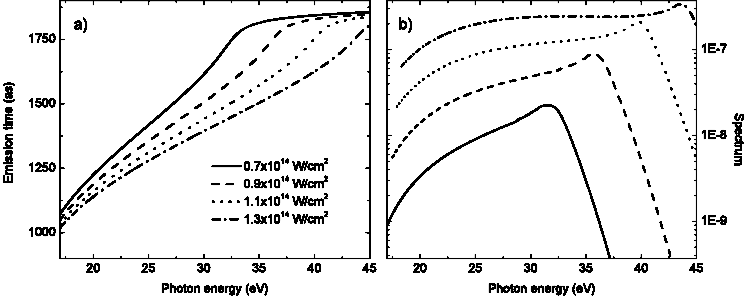
\includegraphics[width=0.8\columnwidth]{Figures/ThreeStep/gdd_argon.pdf}%
\caption{Temps d’émission (gauche) et intensité harmonique (droite) en fonction de l’énergie de photon harmonique et pour différentes intensités de génération. Calcul fait pour l’argon en ne considérant que la trajectoire courte de la GHOE. Tiré de \mycite{DivekiPhD2011}.}
\label{fig:diveki}
\end{figure}

Cette pente linéaire, couramment appelée \textit{atto-chirp}, est donc intrinsèque au mécanisme de génération lui-même \mycite{KazamiasPRA2004}. Elle peut être mesurée expérimentalement, par exemple par la technique RABBIT \mycite{DinuPRL2003,MairesseScience2003}, dont il sera question à la partie \ref{sec:omabbit}. Sa mesure permet également de la compenser, de sorte à comprimer les impulsions attosecondes générées.

\subsection{Phase spatiale des trajectoires quantiques}
\label{sec:phase_spatiale}
Nous avons jusqu'à présent considéré un unique atome émettant un rayonnement harmonique. En réalité, le faisceau de génération a une extension transverse bien plus large qu'un atome, le rayonnement émis est donc la somme cohérente de la contribution de chaque atome unique. Si le faisceau de génération a un profil d'intensité transverse gaussien, son intensité n'est pas uniforme. Nous allons voir que cela se traduit par une phase spatiale non homogène dans l'émission harmonique. On utilise les coordonnées cylindriques $(r,\theta,z)$. En un point $(r,\theta)$ dans le plan transverse, la phase du champ harmonique pour la trajectoire $j$ est donnée par :
\begin{equation}
\phi^j_q = \omega_q t_r - \int_{t_i}^{t_r}\left(\frac{({\bm{p}+\bm{A(t')}})^2}{2}+I_p\right)\rmd t',
\end{equation} 
où $t_i,\;t_r$ et $\bm{p}$ sont les solutions des équations de phase stationnaire. La phase dépend de l'intensité via le potentiel vecteur $\bm{A}(t)$. 

Sur la figure \ref{fig:varju}, tirée de \mycite{VarjuJMO2005}, est tracée $\phi^j_q$ en fonction de l'intensité $I$ pour l'harmonique 19 et pour les deux premières trajectoires quantiques. On observe une dépendance quasiment linéaire, de pente beaucoup plus forte pour la trajectoire longue. Pour les harmoniques loin de l'énergie de coupure, on approxime une dépendance linéaire :
\begin{equation}
\phi^j_q = - \alpha_q^j I,
\label{eq:alphaI}
\end{equation}
où $\alpha_q^j$ est le coefficient de proportionnalité exprimé en $\si{\radian\cm\squared\per\W}$. Cette phase est appelée \textit{phase atomique}. $\alpha_q^{\text{courte}}$ est de l'ordre de $\SI{-1}{\radian\cm\squared\per\W}$ tandis que $\alpha_q^{\text{longue}}\sim\SI{-25}{\radian\cm\squared\per\W}$. Sur le panneau de droite de la figure \ref{fig:varju} est tracé $\partial\phi^j_q/\partial I$ en fonction de l'ordre harmonique. $\alpha_q^{\text{courte}}$ est donc une fonction croissante de l'ordre harmonique, tandis que $\alpha_q^{\text{longue}}$ est décroissante. Dans la coupure, les deux trajectoires se confondent et convergent vers $\approx \SI{-12}{\radian\cm\squared\per\W}$\par
Si on considère maintenant la phase macroscopique du faisceau $\phi^j_q(r,\theta)$ pour une intensité gaussienne, on aura une courbure de phase : la dépendance en intensité du dipôle harmonique modifie la divergence de chaque harmonique. Pour les harmoniques les plus basses, les trajectoires longues auront une divergence bien plus grande que les courtes. Quand l'ordre harmonique augmente, la divergence des trajectoires courtes (resp. longues) augmente (resp. diminue) jusqu'à se confondre à la coupure. Cet effet est bien visible sur les spectres expérimentaux présentés plus loin (figure \ref{Fig:SpectrumGAr}). Il jouera également un rôle central dans la GHOE par un faisceau de Laguerre-Gauss (chapitre \ref{sec:pmodes}).

\begin{figure}[!ht]
\centering
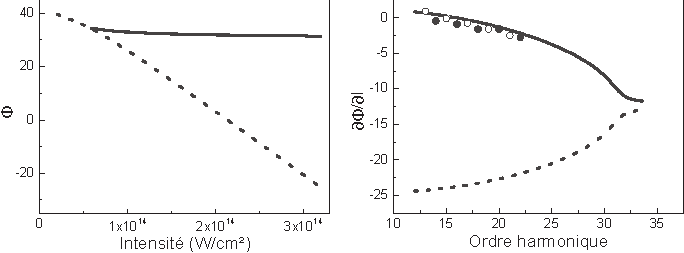
\includegraphics[width=1\columnwidth]{Figures/ThreeStep/alphaI_varju.pdf}%
\caption{Variation de la phase $\phi^j_q$ avec l'intensité (gauche). Le calcul est réalisé pour l'harmonique 19. Variation de $\partial\phi^j_q/\partial I$ avec l'ordre harmonique (droite), à une intensité de $\SI{1.5e15}{\W\per\cm\squared}$. Les lignes continues (resp. pointillées) correspondent aux trajectoires courtes (resp. longues).}
\label{fig:varju}
\end{figure}

\subsection{Accord de phase}
Ces considérations nous amènent à discuter d'un dernier point : l'accord de phase dans la GHOE. Nous avons déjà mentionné que le rayonnement était la somme cohérente de la contribution de chaque atome dans la zone d'interaction. Cette somme doit être réalisé selon la dimension transverse, $(r,\theta)$, et longitudinale, $z$. Si les différentes contributions ne sont pas en phase, des interférences destructives empêcheront l'émission macroscopique de rayonnement XUV. La compréhension de ce phénomène est essentielle pour expliquer les propriétés macroscopiques du rayonnement \mycite{SalieresPRL1995} et pour optimiser le rendement du processus \mycite{KazamiasPRL2003}.

Notons $\bm{k}_q$ le vecteur d'onde de l'harmonique d'ordre $q$ et $\bm{k}_1$ celui du faisceau gaussien de génération. \`A ces deux quantités s'ajoutent des termes de désaccord de phase dus à la phase atomique ainsi qu'à la dispersion électronique et ionique, que l'on note $\Delta \psi_q(r,\theta)$. La condition d'accord de phase pour l'harmonique $q$ s'écrit alors \mycite{BalcouPRA1997} :
\begin{equation}
\bm{k}_q(r,\theta,z) = q\bm{k}_1(r,\theta,z) + \Delta \psi_q(r,\theta,z)
\end{equation}
\mycite{BalcouPRA1997} évaluent le désaccord de phase $|\delta \bm{k}_q| = |\bm{k}_q-q\bm{k}_1 - \Delta \psi_q|$, en négligeant les effets de dispersion sur le laser. La figure \ref{fig:balcou} montre ce désaccord de phase pour les trajectoires courtes et longues. 

\begin{figure}[!ht]
\centering
\includegraphics[width=1\columnwidth]{Figures/ThreeStep/phasematching_balcou.pdf}%
\caption{Désaccord de phase pour les trajectoires longues (gauche) et courtes (droite). Les zones les plus claires indiquent un bon accord de phase. Les pointillés verticaux indiquent les positions des optima de génération d'harmonique. Les flèches représentent la direction d'émission du champ harmonique. Le calcul a été réalisé à une intensité de \SI{6e14}{\W\per\cm\squared} dans le néon, pour l'harmonique 45. Le paramètre confocal est de 5 mm. Tiré de \mycite{BalcouPRA1997}.}
\label{fig:balcou}
\end{figure}

\'Etudions le cas de la trajectoire longue. On observe une structure particulière, en forme de "moustache de morse". On a deux zones notée B et D où le désaccord de phase est minimisé. La zone notée B est située sur l'axe optique mais est très fine, tandis que la zone D est assez étendue et est située en dehors de l'axe optique. De par le volume disponible, la génération d'harmonique proviendra principalement de la zone D. Les flèches indiquent une émission très divergente, ce qui est dû à l'effet de la phase atomique décrit plus haut. Notons également que la zone D se situe en amont de $z=0$, position du foyer du laser de génération. Pour la trajectoire courte (panneau de droite), le comportement est plus simple : on a un maximum du désaccord de phase vers $z\approx-0.5$ mm, qui diminue ensuite dans toutes les directions. Si on s'éloigne trop du foyer laser, l'intensité devient trop faible pour avoir une génération efficace. \mycite{BalcouPRA1997} montrent que l'optimum se situe à $z=3$ mm, où on a un désaccord faible sur un grand volume. 

En conclusion, nous avons mis en évidence deux familles de trajectoires électroniques, qui donnent naissance à deux composantes dans l'émission harmonique ayant des propriétés différentes. Finalement, nous avons vu que l'accord de phase permet de favoriser l'une ou l'autre : la trajectoire courte sera accordée lorsque le foyer optique se situe en amont du jet de gaz, tandis que la longue le sera lorsqu'il se situe en aval. Pour une description plus complète de la théorie de la GHOE, on se reportera à \mycite{ScrinziJPB2006} et à \mycite{SmirnovaIvanov2014}. Le modèle SFA présenté ici est la base des calculs numériques présentés plus loin (partie \ref{sec:sfa}), qui prendront en compte tous les effets de propagation et d'accord de phase dans le milieu. Dans la suite de cette partie, nous expliquons comment réaliser une expérience de GHOE dans le cas habituel d'un faisceau de génération gaussien polarisé linéairement.

\chapter{Aspects expérimentaux de la génération d'harmoniques d'ordre élevé}
\label{Sec:HHG_G}
\section{Système laser}
\label{sec:laser}
Toutes les expériences présentées dans ce chapitre et dans la partie \ref{PA:OAM_HHG} ont été réalisées sur le laser LUCA (Laser Ultra-Court Accordable) du LIDYL au CEA Saclay. Il s'agit d'un laser basé sur la technique "Chirped Pulse Amplification" utilisant le titane saphir comme milieu à gain. Partant d'un oscillateur femtoseconde oscillant autour de 800 nm, le faisceau est étalé temporellement avant d'être amplifié d'abord dans un amplificateur régénératif, puis dans un amplificateur multi-passages. Il est finalement recomprimé dans un compresseur à réseaux \mycite{StricklandOC1985}. La spécificité de ce système est l'insertion récente, juste avant la compression, d'un étage de filtrage modal \mycite{MahieuAPB2015}. Il s'agit d'une fibre creuse de 30 cm de long et $\SI{128}{\micro\metre}$ de diamètre dans laquelle le faisceau est injecté avant d'être collimaté de nouveau. Ceci a pour effet de sélectionner un mode de propagation très proche d'un mode gaussien pur. Finalement on obtient des impulsions dont l'intensité a une enveloppe temporelle gaussienne de largeur à mi-hauteur $\tau = 50$ fs et un profil spatial gaussien de largeur $w_0 = 15$ mm à $\frac{1}{e^2}$. La longueur d'onde utilisée est 792 nm, et l'énergie par impulsion est de 35 mJ pour un taux de répétition de 20 Hz. 

\section{Génération d'harmoniques d'ordre élevé}
Nous commençons par mettre en forme le faisceau laser : son diamètre est ajusté à l'aide d'un iris et son énergie est ajustée grâce à un atténuateur constitué d'une lame demi-onde et d'une paire de polariseurs. \`{A} la sortie de cet atténuateur, la polarisation du laser est verticale (S). Le faisceau est ensuite focalisé par une lentille dans un jet de gaz délivré par une vanne pulsée à la fréquence du laser par un système piezo-électrique (Attotech). L'utilisation d'une vanne pulsée permet de n'envoyer du gaz que lorsque le faisceau laser est présent, ce qui limite la pression résiduelle dans les chambres à vide. Ainsi, on peut atteindre une pression assez élevée ($\simeq$10 mbar) dans la région focale sans que l'émission harmonique ne soit réabsorbée par le gaz résiduel. Un autre paramètre important est le diamètre de l'orifice de la vanne (ici, 150 $\si{\micro\metre}$) : en choisissant un diamètre faible, on crée une extension supersonique du gaz ce qui garantit une longueur d'interaction avec le laser courte dans la direction longitudinale. On s'approche ainsi des conditions idéales d'un plan d'atomes, ce qui limite l'importance des effets d'accord de phase dans la GHOE. \par
Le choix du gaz dépend de l'expérience réalisée : on peut par exemple utiliser une molécule dont on étudie la réponse - c'est le principe de la spectroscopie harmonique. Dans notre cas le gaz n'est pas l'objet d'étude et on préférera utiliser un système simple, facile à se procurer, et ayant une grande section efficace. Le gaz le plus courant est l'argon, qui est peu coûteux et génère de manière très efficace. Son potentiel d'ionisation est de 15.76 eV, ce qui donne une énergie de coupure assez faible et qui empêche de générer des ordres harmoniques très élevés. Dans les cas où on désire générer des ordres élevés et nombreux, on pourra utiliser d'autres gaz rares comme le Néon ($I_p$ = 21.6 eV), bien que la génération soit moins efficace.

Pour notre système, les paramètres nominaux sont :
\begin{itemize}
\item Le diamètre avant focalisation \O{} $\approx$ 10-15 mm,
\item L'énergie par impulsion de l'ordre de E = 1-3 mJ,
\item La lentille de longueur focale f = 1 m. \\
\end{itemize}
Pour connaître la valeur de l'intensité pic au foyer, le profil du faisceau après focalisation peut être calculé numériquement. Le champ avant la lentille est défini dans les coordonnées cylindriques $(R,\theta)$ par :
\begin{equation*}
E(R,\theta) = \sqrt{I_0} \exp{\left(-\frac{R^2}{w_0^2}\right)}\times H(\frac{\mbox{\O}}{2}-R),
\end{equation*}
où $w_0$ est la largeur du faisceau collimaté avant l'iris, \O{}  est le diamètre de l'iris, $H$ est la fonction de Heaviside, et $I_0 = \frac{2E\sqrt{\frac{4\log{2}}{\pi}}}{\tau\pi w_0^2}$.
La focalisation d'un faisceau par une lentille mince peut être calculée par une transformée de Fourier (voir \mycite{Goodman}, un des ouvrages de référence pour l'optique de Fourier, et \mycite{Tan} pour des exemples d'implémentations numériques). Ces calculs permettent d'étudier l'influence des différents paramètres. Par exemple, on peut faire varier le diamètre de l'iris : la Figure \ref{Fig:IrisScan} montre le profil du faisceau au foyer quand \O{} varie entre 5 et 25 mm. On voit alors que l'intensité pic au foyer part d'une valeur $<10^{13}$ et monte jusqu'à $\SI{10e14}{W/cm^2}$. On se trouve donc parfaitement dans le régime d'intensité nécessaire à la génération d'harmonique : l'intensité est suffisante pour enclencher une ionisation tunnel mais reste assez faible pour ne pas ioniser et dépléter tout le milieu.

\begin{figure}[!ht]
\centering
\def\svgwidth{\columnwidth}
\import{Figures/Iris_Scan/}{Fig_IrisScan.pdf_tex}
\caption{\'{E}volution du foyer lorsqu'on varie la taille de l'iris. De gauche à droite : (1) profil transverse de l'intensité au foyer, (2) intensité pic, (3) taille du waist. Les paramètres sont les suivants : E = 1 mJ, $w_0$ = 15 mm, $\tau$ = 50 fs, $\lambda$ = 792 nm, f = 1 m et \O{} variant de 5 à 25 mm par pas de 1 mm. Le calcul est réalisé sur une grille de 1025x1025 points correspondant à une taille réelle de 5*\O{}.}
\label{Fig:IrisScan}
\end{figure}

Les harmoniques d'ordre élevé du laser infrarouge sont ainsi générées par le gaz injecté près du foyer de la lentille. Pour leur détection et caractérisation, nous avons utilisé d'une part un spectromètre électronique à temps de vol, d'autre part un spectromètre de photons. Le premier requiert un rayonnement focalisé alors que le second accepte en entrée un rayonnement divergent. Afin de pouvoir utiliser ces deux diagnostics successivement, avant d'entrer dans le spectromètre, le rayonnement XUV est ré-imagé par un dispositif composé de deux optiques (représentées plus bas sur la figure \ref{Fig:ExpG}) :
\begin{enumerate}
\item Un miroir torique en or de 50 cm de focale. Le miroir travaille à $11.5\degres$ d'incidence rasante ($78.5\degres$ par rapport à la normale au miroir), ce qui permet d'avoir une réflectivité importante et plate sur la gamme spectrale considérée (voir Figure \ref{Fig:TorR}).

\begin{figure}[!ht]
\centering
\def\svgwidth{0.6\columnwidth}
\import{Figures/Reflect_Torique/}{torR.pdf_tex}
\caption{Réflectivité calculée du miroir torique en or à un angle d'incidence de $11.5\degres$. (CXRO, \mycite{Henke1993}).}
\label{Fig:TorR}
\end{figure}
Le miroir torique est utilisé dans une configuration 2f-2f de sorte à garder un rapport\shorthandoff{:} 1:1 \shorthandon{:}entre le foyer de génération et le second foyer. \`{A} la position de ce second foyer nous pouvons placer le spectromètre à temps de vol, qui sert dans le cas d'une mesure RABBIT (voir la partie \ref{sec:omabbit}). Un autre avantage de cette imagerie est d'éloigner la zone de génération, où la pression est élevée, du spectromètre de photons, qui requiert un vide de l'ordre de $10^{-5}$ mbar pour que les détecteurs fonctionnent.\\

\item La deuxième optique est une lame de Si$\mbox{O}_{\mbox{2}}$, qui joue le rôle de filtre de l'infrarouge de génération. La lame de silice est traitée antireflet pour l'infrarouge grâce à un dépôt multicouches. La dernière de ces couches est en silice, ce qui, combiné à une bonne qualité de surface permet de réfléchir efficacement le rayonnement harmonique. La Figure \ref{Fig:SilR}, tirée de \mycite{MairessePhD}, présente la réflectivité de la lame pour le rayonnement harmonique et infrarouge. La réflectivité dans l'extrême ultra violet (XUV) est donc supérieure à 50\% jusqu'à l'ordre $\approx 37$, tandis que moins de 10\% de l'infrarouge est réfléchi. Le filtrage de l'infrarouge de génération est souvent crucial : il constitue un bruit de mesure non négligeable, sans compter qu'il peut facilement endommager des optiques ou des détecteurs en aval s'il est focalisé.

\begin{figure}[!ht]
\centering
\def\svgwidth{\columnwidth}
\import{Figures/Reflect_Silice/}{silR.pdf_tex}
\caption{Réflectivité de la lame de silice. \`{A} gauche, transmission et réflectivité à 800 nm en fonction de l'angle d'incidence rasante. Les pointillés repèrent notre angle de $11.5\degres$. \`{A} droite, réflectivité XUV mesurée (cercles bleus) et donnée par le CXRO (ligne violette) (\mycite{Henke1993}). Figure adaptée de \mycite{MairessePhD}.}
\label{Fig:SilR}
\end{figure}
\end{enumerate}

Comme nous le verrons plus loin, pour l'étude des faisceaux de Laguerre-Gauss, il sera crucial d'imager le spectre harmonique, c'est-à-dire de séparer les différents ordres harmoniques et de mesurer leurs propriétés spatiales. C'est le rôle du spectromètre de photons. Environ 50 cm en aval du second foyer, les harmoniques sont dispersées par un réseau à pas variable cylindrique Hitachi 001-0437 (voir \mycite{KitaAO1983} pour des détails sur son fonctionnement). Comme pour les réseaux à pas fixe, l'angle de réflexion d'un rayonnement monochromatique de longueur d'onde $\lambda$ est donné par la formule :
\begin{equation*}
m\lambda=\frac{\sin{\alpha}+\sin{\beta}}{\sigma},
\end{equation*}
où $m$ est l'ordre de diffraction considéré (généralement 1), $\sigma$ le nombre de trait par mètre (1200 traits/mm dans notre cas), $\alpha$ et $\beta$ les angles d'incidence et de réflexion, définis par rapport à la normale au réseau (la documentation donne $\alpha = 87$\degres{} pour un fonctionnement optimal).\par
Le réseau de diffraction est cylindrique, le rendant focalisant uniquement dans la dimension horizontale. Un rayonnement gaussien de faible largeur spectrale $\Delta\lambda$ et de largeur spatiale $w(z)$ formera donc dans le plan focal du réseau une fine ligne verticale de largeur proportionnelle à $\Delta\lambda$ et de hauteur $w(z)$. On image ainsi à la fois les dimensions spectrale et spatiale, si on suppose la symétrie cylindrique. Ce spectre est imagé par des galettes de micro-canaux couplées à un écran de phosphore, lui-même observé par une caméra CCD Basler A102f. 

L'intégralité du dispositif expérimental est représenté sur la Figure \ref{Fig:ExpG}.

\vspace{\baselineskip}
\begin{figure}[!ht]
\centering
\def\svgwidth{\columnwidth}
\import{Figures/Setup_G/}{setupG_wbitmap.pdf_tex}
\caption{Dispositif expérimental de génération et détection d'harmoniques d'ordre élevé.}
\label{Fig:ExpG}
\end{figure}

Les figures \ref{Fig:SpectrumGAr} et \ref{Fig:SpectrumGNe} présentent des spectres obtenus avec ce dispositif en utilisant respectivement l'argon et le néon comme gaz de génération. On observe les ordres harmoniques allant de 13 à 29 dans l'argon, et de 13 à 57 dans le néon. Le potentiel d'ionisation du Néon, plus élevé que celui de l'argon, a permis d'utiliser une intensité plus importante sans ioniser complètement le milieu. Conformément à la loi de coupure on obtient dans ce cas un spectre plus étendu. Sur le spectre de l'argon, on observe clairement les deux premières trajectoires quantiques de la GHOE (voir partie \ref{sec:thTraj}) : une contribution sur l'axe correspond à la trajectoire courte et une plus divergente et moins intense correspond à la trajectoire longue. Dans le cas du néon, les conditions d'accord de phase utilisées favorisent la trajectoire courte. On remarque également que la divergence de la trajectoire courte (resp. longue) augmente (rep. diminue) avec l'ordre harmonique, jusqu'à ce que les deux trajectoires se confondent dans la coupure. Notons finalement la présence sur le spectre du néon de pics satellites autour des harmoniques les plus basses : il s'agit des harmoniques plus élevées diffractées au second ordre par le réseau.
\begin{figure}[!ht]
\centering
\def\svgwidth{\columnwidth}
\import{Figures/Spectrum_G/}{Spectrum_G_Ar.pdf_tex}
\caption{Spectre d'harmoniques d'ordre élevé générées dans l'argon à partir d'un mode laser gaussien.}
\label{Fig:SpectrumGAr}
\end{figure}
\begin{figure}[!ht]
\centering
\def\svgwidth{\columnwidth}
\import{Figures/Spectrum_G/}{Spectrum_G_Ne.pdf_tex}
\caption{Spectre d'harmoniques d'ordre élevé générées dans le néon à partir d'un mode laser gaussien.}
\label{Fig:SpectrumGNe}
\end{figure}
